\section{Generatorul echivalent de tensiune}

\begin{figure}
\begin{center}
\begin{circuitikz}[scale=1.4,european resistors,american inductors]
\draw (0,0) -- (0,2) to[R, l = $R_1$, *-*] (4,2) to[R, l = $R$] (4,0) to[romanianVoltageSource, l = $E_e$] (0,0);
\end{circuitikz}
\caption{Generatorul Echivalent $E_e = E_5 + J_4R_2 = 7V$ Rezistenta echivalenta $R = 3\Omega$}

\label{fig:circusgay}
\end{center}
\end{figure}


Circuitul cu generatorul echivalent este in Fig \ref{fig:circusgay}.
Am ales sa variez rezistenta intre 0 si $5\Omega$ pentru a surprinde transferul maxim de putere. Am marcat cu o steluta rosie conditiile initiale si cu o steluta verde conditiile de transfer maxim de putere.

\begin{figure}
\begin{center}
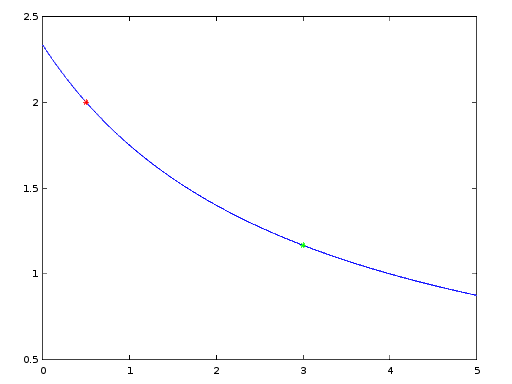
\includegraphics[width=0.6\textwidth]{intensitate.png}
\caption{grafic $I(R)$}
\end{center}
\end{figure}

\begin{figure}
\begin{center}
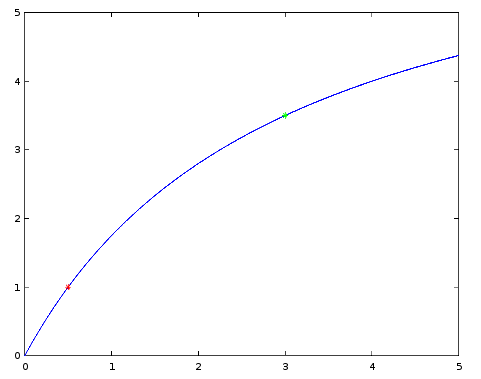
\includegraphics[width=0.6\textwidth]{tensiune.png}
\caption{grafic $U(R)$}
\end{center}
\end{figure}

\begin{figure}
\begin{center}
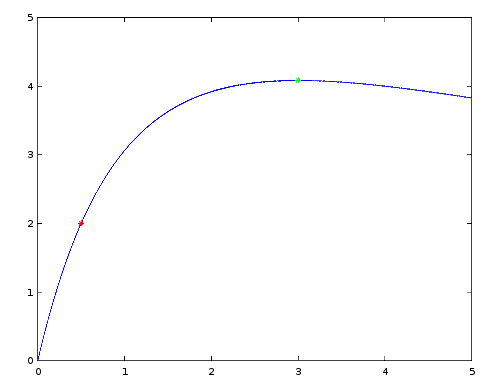
\includegraphics[width=0.6\textwidth]{putere.png}
\caption{grafic $P(R)$}
\end{center}
\end{figure}

\begin{figure}
\begin{center}
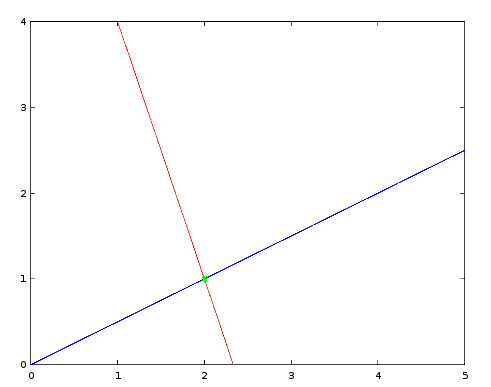
\includegraphics[width=0.6\textwidth]{pstatrez.png}
\caption{grafic $U(I)$ pentru rezistor liniar(albastru)}
\label{fig:pstatrez}
\end{center}
\end{figure}

In Fig \ref{fig:pstatrez} se poate observa ca punctul static de functionare este exact acelasi ca cel care a reiesit din calcul la subpunctul 1. Dioda semiconductoare poate fi orientata in directia pozitiva a curentului, sau in directia opusa, am ales sa orientez dioda in directia pozitiva a curentului din Fig \ref{fig:circusgay}, pentru ca altfel ar fi functionat aproximativ ca un izolator perfect.

\begin{figure}
\begin{center}
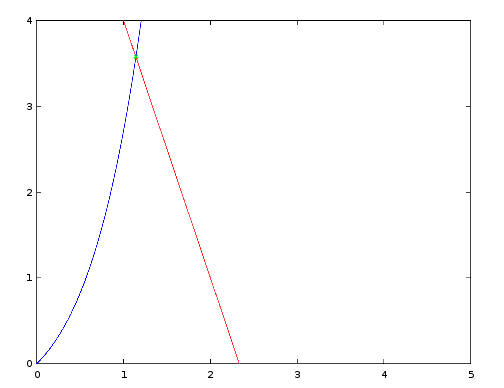
\includegraphics[width=0.6\textwidth]{pstatdioda.png}
\caption{grafic $U(I)$ pentru dioda(albastru)}
\end{center}
\end{figure}


\newpage
\begin{lstlisting}
r = 3;
E = 7;
Ri = 0.5;
R = linspace(0, 5, 1e5);
Rmax = r;

figure(1);
hold on;
plot(R, E * E * R ./ ((R + r) .^ 2));
plot(Ri, E * E * Ri ./ (r + Ri) .^ 2, 'r*');
plot(Rmax, E * E * Rmax ./ (r + Rmax) .^ 2, 'g*');

figure(2);
hold on;
plot(R, E ./ (r + R));
plot(Ri, E ./ (r + Ri), 'r*');
plot(Rmax, E ./ (r + Rmax), 'g*');

figure(3);
hold on;
plot(R, E * R ./ (r + R));
plot(Ri, E * Ri ./ (r + Ri), 'r*');
plot(Rmax, E * Rmax ./ (r + Rmax), 'g*');

I = linspace(0, 5, 1e5);
D = I;
D = e .^ D;

figure(4); hold on;
plot(I, I * Ri, '-b');
plot(I, 7 - I * r, '-r');
plot(2, 1, 'g*');
ylim([0 4]);

pstat = 1.1416;

figure(5); hold on;
plot(I, I .* D, '-b');
plot(I, 7 - I * r, '-r');
plot(pstat, pstat*e^pstat, 'g*');
ylim([0 4]);
\end{lstlisting}
